\documentclass{lxaiproposal}


%   \usepackage[english,french]{babel}   % "babel.sty" + "french.sty"
\usepackage[english]{babel}   % "babel.sty" + "french.sty"

% \usepackage[english,francais]{babel} % "babel.sty"
% \usepackage{french}                  % "french.sty"
\usepackage{times}            % ajout times le 30 mai 2003

\usepackage{epsfig}
\usepackage{graphicx}
\usepackage{booktabs}
\usepackage{multirow}
\usepackage{pifont}
\usepackage{caption}
\usepackage{subcaption}

\usepackage{amsmath}
\usepackage{mathtools}
\usepackage{amssymb}
\usepackage{algorithm}
\usepackage[noend]{algpseudocode}


\usepackage{array}
\usepackage{color}
\usepackage{colortbl}

\usepackage{pifont}
\usepackage{amssymb}
\usepackage{latexsym}

\usepackage{booktabs}

%% --------------------------------------------------------------
%% FONTS CODING ?
% \usepackage[OT1]{fontenc} % Old fonts
% \usepackage[T1]{fontenc}  % New fonts (preferred)
%% ==============================================================

\title{ECSE 6810 Final Project \\ DAG Structure Learning using Generative Flow Networks}

\author{\coord{Ali}{Najibi}{}\\\\
\coord{\textbf{Course Instructor: Prof. Qiang}}{\textbf{Ji}}{}
}

\address{\affil{}{Rensselaer Polytechnic Institute}
}

%% If all authors have the same address %%%%%%%%%%%%%%%%%%%%%%%%%%%%%%%%%%%%%%%
%                                                                             %
%   \auteur{\coord{Michel}{Dupont}{},                                         %
%           \coord{Marcel}{Dupond}{},                                         %
%           \coord{Michelle}{Durand}{},                                       %
%           \coord{Marcelle}{Durand}{}}                                       %
%                                                                             %
%   \adress{\affil{}{Laboratoire Traitement des Signaux et des Images \\      %
%     1 rue de la Science, BP 00000, 99999 Nouvelleville Cedex 00, France}}   %
%                                                                             %
%                                                                             %
%%%%%%%%%%%%%%%%%%%%%%%%%%%%%%%%%%%%%%%%%%%%%%%%%%%%%%%%%%%%%%%%%%%%%%%%%%%%%%%

\email{}

\englishabstract{
    Directed Acyclic Graphs (DAGs) are widely used in modeling complex systems where relationships are directional
    and non-cyclic. Using these graphs, we can model complex distributions and perform inference tasks. There are
    multiple algorithms to learn the structure of a DAG from data including ......}

\begin{document}

    \maketitle
    \\


    \section{Introduction}
    \vspace*{-3mm}

    Bayesian Networks (BNs) are powerful tools for modeling complex systems where relationships are directional and
    non-cyclic. A BN consists of a DAG $G$ where each node represents a random variable and edges
    represent the conditional dependencies between the variables. Moreover, each BN has a set of parameters $\theta$ that
    represent the conditional probability distributions of each variable given its parents.

    The Major characteristic of BNs that make them extremely useful in modeling probability distributions is the
    conditional independence property. This property states that a variable $X$ is conditionally independent of its
    non-descendants given its parents. This property allows us to factorize the joint probability distribution of the
    variables in the graph as follows:
    \begin{equation}
        P(X_1, X_2, \ldots, X_n) = \prod_{i=1}^{n} P(X_i | \text{Pa}(X_i))
        \label{eq:bn_factorization}
    \end{equation}
    where $\text{Pa}(X_i)$ denotes the parents of variable $X_i$ in the graph.

    Learning a target distribution $P(X)$ from data $D$ is a fundamental problem in machine learning. In the context of
    BNs, this problem is to learn the structure of the DAG $G$ and the parameters $\theta$ that best represent the
    distribution $P(X|D)$. To achieve that, we can factorize $P(X|D)$ as:
    \begin{equation}
        P(X|D) = \sum_{G} P(G|D) P(\theta|G,D) P(X|G,\theta,D)
        \label{eq:bn_learning}
    \end{equation}
    where $P(G|D)$ is the posterior distribution of the DAG given the data, $P(\theta|G,D)$ is the posterior distribution
    of the parameters given the DAG and the data, and $P(X|G,\theta,D)$ is the likelihood of the data given the DAG and
    the parameters.


    A central problem in Bayesian Networks is structure learning — identifying the DAG $G$ and parameters
    $\theta$ that best explain the observed data $D$. This process typically involves approximating the posterior
    distribution $P(G\mid D)$, a computationally intensive task due to the combinatorial nature of
    possible DAGs. Conventional methods like Markov Chain Monte Carlo (MCMC) and Variational Inference address this
    challenge but often face limitations such as slow convergence and computational inefficiencies.

    Generative Flow Networks (GFlowNets)~\cite{bengio2023gflownetfoundations}, recently introduced as a novel
    probabilistic modeling paradigm, can be leveraged to model this distribution as a sequential decision-making
    problem. By treating DAG construction as a sequential decision-making problem, GFlowNets approximate the
    posterior $P(G\mid D)$ by sampling DAGs through learned transition probabilities. This approach provides notable
    advantages over traditional methods, including improved scalability and guaranteed adherence to acyclicity
    constraints. To this end, we w

    In this project, we want to explore the potential of GFlowNets in learning the structure of a DAG from data. We
    will implement the proposed approach in the original paper~\cite{deleu2022daggflownet} and evaluate its performance
    on synthetic data. We will compare the results using various evaluation metrics including SHD, E-SHD, Ancestor
    Relationship, and BGe score.
    .......

    The following sections of this report are organized as follows. In Section~\ref{sec:related_work}, we provide a
    brief overview of the related work including the main algorithms used in for learning $\P(G|D)$. Then, we proceed
    to describe the main concepts and algorithms used in this project in Section~\ref{sec:background}. In Section~\ref{sec:proposed_approach},
    we describe the proposed approach for learning the structure of a DAG using generative flow networks in the
    original paper~\cite{deleu2022daggflownet}. Later we will describe and comprehensively explain the experiments
    conducted in this project in Section~\ref{sec:experiments} along with the results of the
    experiments. Finally, we will conclude the report in Section~\ref{sec:conclusion}
    followed by Section~\ref{sec:future_work} where we will discuss the future work.


    \section{Related Work}\label{sec:related_work}
    \vspace*{-3mm}

    In this section, we provide a brief overview of the main algorithms used for learning the structure of a DAG from
    data.

    \subsection{Markov Chain Monte Carlo (MCMC)}
    \vspace*{-3mm}
    The process of learning a posterior distribution $P(G|D)$ is computationally intensive; thus, the first idea that
    comes to mind is to sample from this distribution instead of completely learning it. Markov Chain Monte Carlo (MCMC)
    is the most effective and widely used method for sampling method. MCMC methods are based on the idea of constructing
    a Markov chain that has the desired distribution as its stationary distribution. Multiple approaches~\cite{
        mcmc1, mcmc2, mcmc3} have been proposed to sample from the posterior distribution of the DAG given the data.
    However, these methods are computationally expensive and often face limitations such as slow convergence and
    computational inefficiencies. Recently in~\cite{viinikka2020scalablebayesianlearningcausal}, Viinikka et al. proposed a scalable approach towards
    learning the structure of a DAG using MCMC methods.

    \subsection{Variational Inference}
    \vspace*{-3mm}

    Variational Inference (VI) is another popular method for approximating the posterior distribution $P(G|D)$. VI
    methods are based on the idea of approximating the posterior distribution with a simpler distribution that is easier
    to sample from. Methods leveraging this approach mostly use Gradient-based methods to minimize the difference
    between the true posterior and the approximated posterior. In~\cite{cundy2021bcdnetsscalablevariational}, Cundy et al. proposed a scalable
    approach for learning the structure of a DAG using Variational Inference; they tried to address the limitation
    decomposing the adjacency matrix into a triangular matrix and a permutation. Other methods like~\cite{annadani2021variationalcausalnetworksapproximate, lorch2021dibsdifferentiablebayesianstructure}
    try to relax the acyclicity constraint into a soft prior $P(G)$ considering continuous acyclicity.


    \section{Background}\label{sec:background}
    \vspace*{-3mm}

    The problem of learning the structure of a DAG from data could be formulated as learning the transition probabilities
    of a Markov Chain where each state represents a DAG. In such a formulation, the goal is to learn these
    transition probabilities such that the probability of seeing each state is proportional to the posterior probability
    of the DAG given the data. This process could be modeled as a sequential decision-making problem.
    DAG-GFlowNet~\cite{deleu2022daggflownet} is a novel approach that leverages Generative Flow Networks (GFlowNets) to
    model $P(G|\mid D)$.

    \subsection{Generative Flow Networks}
    \vspace*{-3mm}

    Suppose we have a sampling space $\mathcal{X}$ and a target distribution $P(X)$. The goal of Generative Flow
    Networks (GFlowNets) is to model this distribution by generating samples $X \in \mathcal{X}$ with probabilities
    proportional to a given reward function $R(X)$, such that $P(X) \propto R(X)$. To achieve this, GFlowNets treat
    the generation of samples as a sequential decision-making process over a Directed Acyclic Graph (DAG) of states.

    GFlowNet has an internal DAG of states $s \in \mathcal{S}$, where each state represents a partial or complete
    sample, starting from an initial state $s_0$ and terminating at a special absorbing state $s_f$. Note that only
    complete states are connected to the absorbing state.

    Transitions between states are guided by learned
    probabilities, and the task is to ensure that the flow of probabilities through the states satisfies the
    \textit{flow-matching condition}~\eqref{eq:flow_matching} at each state $s \in \mathcal{S}$. This condition
    ensures that the total incoming flow to a state equals the outgoing flow plus the reward at that state.

    \begin{equation}
        \sum_{s \in \text{Pa}(s')} F(s \to s') = \sum_{s'' \in \text{Ch}(s')} F(s' \to s'') + R(s'),
        \label{eq:flow_matching}
    \end{equation}

    where $F(s \to s')$ is the flow between states $s$ and $s'$, and $\text{Pa}(s')$ and $\text{Ch}(s')$ are the
    parent and child states of $s'$, respectively. Note that the $R(s) = 0$ for any incomplete state
    $s \in \mathcal{S}\setminus\mathcal{X}$ and is positive for complete states $s \in \mathcal{X}$.

    If the flow-matching condition~\eqref{eq:flow_matching} is satisfied, GFlowNet induces a generative process to
    sample complete states $s \in \mathcal{X}$ with probability proportional to the reward function $R(s)$. In other
    words, starting from the initial state $s_0$, the generative process will traverse the DAG of states, sampling
    each state $s_i$ using the transition probabilities defined as normalized outgoing flows consistent with~\eqref{eq:flow_prob}.

    \begin{equation}
        P(s_{i+1} \mid s_i) \propto F(s_i \to s_{i+1}),
        \label{eq:flow_prob}
    \end{equation}

    This process, will result in a sample $s$ with probability $P(s) \propto R(s)$. In other words, consider~\eqref{eq:flow_matching} equation, there are two explanations for a high reward $R(s)$: either the flow from the parent
    states is high or the flow to the child states is low. This is the key idea behind GFlowNets.


    \textbf{Detailed-Balance Condition} One challenge that exists in formulating the flow-matching condition is that it
    tends to be orders of magnitude larger as we get closer to the intial state --- this is due to the fact that the
    initial state scaters the whole flow of the network and thus, contains $\sum_{s \in \mathcal{X}} R(s)$ flow.

    Such difference in flow values makes it difficult to parametrize $F$. Authors used proposed alternative by Bengio
    et al. in~\cite{bengio2023gflownetfoundations} to address this issue. This approach suggests parametrization of
    forward and backward transition probabilities $P_{\phi}(s_{i+1} \mid s_i)$ and $P_{\psi}(s_i \mid s_{i+1})$ such
    that the flow-matching condition is satisfied through Eq.~\eqref{eq:detailed_balance}.

    This equation --- proof could be seen in Appendix~\ref{app:detailed_balance} --- holds in the case that all states of the GFlowNet are
    complete (except the terminal state $s_f$). Moreover, $P_{\phi}(s_{i+1} \mid s_i)$ is an encoding of the forward
    flow --- a distribution over the child states of $s_i$ --- and $P_{\psi}$ is an encoding of the backward flow --- a
    distribution over the parent states of $s_{i+1}$. Eq.~\eqref{eq:detailed_balance} ensures that the flow-matching
    condition holds for any transition $s_i \to s_{i+1}$.

    \begin{equation}
        \begin{aligned}
            R(s_i) P_{\phi}(s_{i+1} \mid s_i)P_{\phi}(s_f \mid s_{i+1})=\\
            R(s_{i+1}) P_{\psi}(s_i \mid s_{i+1})P_{\phi}(s_f \mid s_i)
        \end{aligned}
        \label{eq:detailed_balance}
    \end{equation}


    \section{Proposed Approach}\label{sec:proposed_approach}

    \subsection{GFlowNet for DAG Structure Learning}

    The proposed approach in~\cite{deleu2022daggflownet} leverages Generative Flow Networks (GFlowNets) to model the
    posterior distribution $P(G|D)$ of a DAG given data $D$. The goal is to learn the transition probabilities of a
    Markov Chain where each state represents a valid DAG$G$.

    To further elaborate this notion, first, let's take a look at Fig.~\ref{fig:dag_gflownet}. This figure shows the
    overall generation process of a DAG using GFlowNet. The process starts from an initial state $G_0$ and moves
    forward, according to the transition probabilities, $P_{\phi}(G_{i+1} \mid G_i)$ until it reaches the absorbing state
    $s_f$. Note that since in Eq.~\eqref{eq:detailed_balance} we assumed that all states are complete except the
    absorbing state, all states of the inner DAG of GFlowNet should be valid DAGs (except the absorbing state).
    At each step, moving from $G_i$ to $G_{i+1}$, we add an edge to the DAG considering the acyclicity constraint.
    The aciclicity constraint is enforced using some masking operation on the adjacency matrix of the DAG which is
    explained in details in Appendix~\ref{app:masking}.


    \begin{figure}[h]
        \centering
        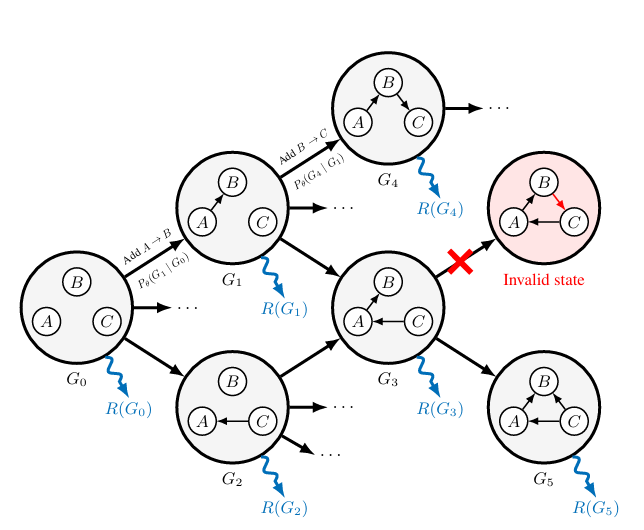
\includegraphics[width=0.5\textwidth]{figures/dag_gflownet}
        \caption{DAG-GFlowNet: Generative Flow Network for DAG Structure Learning for 3 nodes. Figure taken from~\cite{deleu2022daggflownet}.}
        \label{fig:dag_gflownet}
    \end{figure}

    To parameterize the forward transition probabilities $P_{\phi}(G_{i+1} \mid G_i)$, the authors have distinguished
    between two types of transition, terminating transition $P_{\phi}(s_f \mid G_i)$ and non-terminating transition
    $P_{\phi}(G_{i+1} \mid G_i)$.
    More accurately, the non-terminating transition should be written as:
    \begin{equation}
        P_{\phi}(G_{i+1} \mid G_i) = (1-P_{\phi}(s_f \mid G_i)) P_{\phi}(G_{i+1} \mid G_i, \neg s_f)
        \label{eq:non_terminating_transition}
    \end{equation}
    where $P_{\phi}(G_{i+1} \mid G_i, \neg s_f)$ is the transition probability from $G_i$ to $G_{i+1}$ knowing we do not
    terminate.

    Simply put, $G_{i+1}$ is the result of adding an edge to $G_i$, thus, $P_{\phi}(G_{i+1} \mid G_i, \neg s_f)$ can
    be modeled
    as a probability distribution over all the possible moves $d^2$ --- where $d$ is the number of nodes in the graph ---
    that can be made to $G_i$ to get $G_{i+1}$. However, to account for the acyclicity constraint, the authors have
    proposed filtering out actions not leading to valid DAGs and setting their probabilities to zero. Then, normalizing
    the remaining probabilities to sum to one.

    \subsection{Neural Network Architecture}\label{sec:nn_architecture}
    \vspace*{-3mm}

    Eq.~\eqref{eq:non_terminating_transition} suggests that the transition probabilities could be modeled using the
    same backbone with $\phi$ as the parameters and different heads in the output layer. The authors used a neural
    network to satisfy: (1) invariant to the order of the input, since each state is represented as a set of edges,
    (2) transform a set of input edges into a set of output probabilities for each edge to be added, and (3) bounded
    parameters despite the unbounded nature of the input, specifically $d$ --- the number of nodes in the graph.

    One choice to satisfy these requirements would be to use transformers~\cite{vaswani2023attentionneed}, however,
    because of the size of the input, $d^2$, the self-attention layers would scale up to $O(d^4)$, which makes it
    interactable for large graphs. Instead, authors used a Linear Transformer~\cite{katharopoulos2020transformersrnnsfastautoregressive}.
    Detailed explanation of linear attention mechanism could be found in Appendix~\ref{app:linear_attention}.

    This concludes us to the architecture of the neural network used in the proposed approach. Fig.~\ref{fig:nn_architecture}
    shows the overall architecture of the neural network used in the proposed approach.

    \begin{figure*}
        \centering
        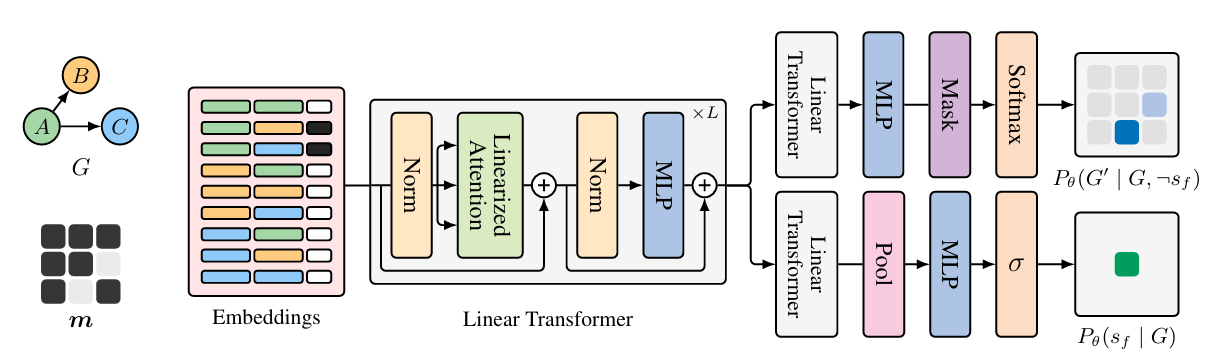
\includegraphics[width=0.92\textwidth]{figures/nn_architecture}
        \caption{Neural Network Architecture used in the proposed approach.
        The input Graph $G$ is embedded into an embedding of $d^2$ edges where each edge is itself embedded using
        embedding of its outgoing and incoming nodes along with an indicator of its presence in the graph. A linear Transformer
        with $L$ layers is used and the output is passed through two different heads to copmute the terminating and non-terminating
        forward transition probabilities. Note that for $P_{\phi}(G_{i+1} \mid G_i, \neg s_f)$, the output is passed through a
        masking later filtering out invalid actions before using a softmax layer to normalize the probabilities. Figure taken from~\cite{deleu2022daggflownet}.}
        \label{fig:nn_architecture}
    \end{figure*}

    \vspace*{3mm}

    \textbf{The loss function} Now that we have defined the overall architecture of the neural network and the
    transition probabilities, we need to define the loss function to train the network.
    To satisfy Eq.~\eqref{eq:detailed_balance}, authors suggested using the following loss function:
    \begin{equation}
        \begin{array}{l}
            \mathcal{L}(\phi) = \\
            \sum_{G_i \to G_{i+1}} \left[ \log
            \frac{R(G_{i+1})P_{\psi}(G_i \mid G_{i+1})P_{\phi}(s_f \mid G_i)}{R(G_i)P_{\phi}(G_{i+1} \mid G_i)P_{\phi}(s_f \mid G_{i+1})} \right]^2 .
        \end{array}
        \label{eq:loss_function}
    \end{equation}

    Note that this loss function is defined as a function of $\phi$ and not $\psi$. This is because the backward
    transition is considered to be fixed and not learned.

    \subsection{Bayesian Structure Learning using GFlowNet}

    Suppose we are given a dataset $\mathcal{D} = \{x^{(1)}, x^{(2)}, \ldots, x^{(N)}\}$ where each $x^{(i)}$ is an i.i.d
    fully observed sample from the target distribution. The goal is to obtain a posterior distribution
    $P(G|\mathcal{D})$.
    As mentioned before, GFlowNet models a distribution $P(s) \propto R(s)$, now if we define the reward function $R(s)$
    according to Eq.~\eqref{eq:reward_function}, we can model the posterior distribution $P(G|\mathcal{D})$ using
    GFlowNet.
    \begin{equation}
        R(s) = P(G|D) = P(G)P(D|G) = P(G) P(\theta|G) P(D|\theta, G)
        \label{eq:reward_function}
    \end{equation}
    where $P(G)$ is the prior distribution of the DAG and $P(D|G)$ is the likelihood of the data given the DAG.

    The authors tried to make the reward function modular and thus, computationally efficient. They assumed that both the
    prior $P(G)$ and the prior over the parameters $P(\theta|G)$ are modular, thus, choosing a modular likelihood
    function can result in a modular reward function. BGe score~\cite{geiger2021learninggaussiannetworks} and
    BDe score~\cite{heckerman2015learningbayesiannetworkscombination} are two examples of modular likelihood functions that
    were used by the authors in their experiments.

    Considering modularity we have:
    \begin{equation}
        \log R(G) = \sum_{j=1}^{d} LocalScore(X_j, \text{Pa}_G(X_j)).
        \label{eq:modular_reward}
    \end{equation}

    This will yield Eq.~\eqref{eq:log_diff} for adding edge $X_i \to X_j$ to the graph $G$ resulting in graph $G'$.

    \begin{equation}
        \begin{aligned}
            \log \frac{R(G')}{R(G)} &= \log R(G') - \log R(G) =\\
            & = \text{LocalScore}(X_j \mid \text{Pa}_{G}(X_j)\cup \{X_i\}) \\
            &-\text{LocalScore}(X_j \mid \text{Pa}_{G}(X_j)).
        \end{aligned}
        \label{eq:log_diff}
    \end{equation}

    This difference in local scores is called the \textit{delta score} in the paper. The authors used the delta score.

    \subsection{Learning a large DAG space}
    \vspace*{-3mm}

    As the DAG space is combinatorial, in the learning process, we cannot account for all possible graphs in the
    space. To address this challenge, the authors took advantage of an \textbf{RL} approach called \textbf{
        Off-Policy Learning}

    The idea is to buffer transitions from the generative process and use them to train the neural network in future
    steps. Suppose for any transition $G \to G'$, we buffer the transition in some buffer $\mathcal{B}$.
    Then, we can use the transitions in $\mathcal{B}$ with respect to some distribution $\pi$ to minimize:
    \begin{equation}
        \mathcal{L}(\phi) = \mathbb{E}_{\pi} \left[ \left[ \log
        \frac{R(G')P_{\psi}(G \mid G')P_{\phi}(s_f \mid G)}{R(G)P_{\phi}(G' \mid G)P_{\phi}(s_f \mid G')} \right]^2 \right].
        \label{eq:off_policy_loss}
    \end{equation}

    Inspired by reinforcement learning again, the distribution $\pi$ could be learned on-policy as
    $P_{\phi}(G' \mid G)$ and used off-policy during the learning process. This is kind of similar to the \textit{
        Expectation Maximization}~\cite{dempster1977maximumlikelihood} algorithm where the E-step is done on-policy and
    the M-step is done off-policy.
    All that said, the authors used a variant of the \textbf{Q-learning} algorithm to learn the distribution $\pi$.
    The Q-learning algorithm is used to learn the optimal policy $\pi$ that maximizes the expected reward.

    To end this section, we can summarize the proposed approach in Algorithm~\ref{alg:proposed_approach}.
    \begin{algorithm}
        \caption{Proposed Approach for Learning the Structure of a DAG using GFlowNet}
        \label{alg:proposed_approach}
        \begin{algorithmic}[1]
            \State Initialize the neural network parameters $\phi$.
            \State Initialize the buffer $\mathcal{B}$.
            \State Fill the buffer $\mathcal{B}$ with some initial transitions along with their delta scores.
            \While{not converged}
                \State Sample a batch of transitions from $\mathcal{B}$.
                \State Compute the loss function $\mathcal{L}(\phi)$ using Eq.~\eqref{eq:log_diff} and Eq.~\eqref{eq:off_policy_loss}.
                \State Update the neural network parameters $\phi$ using the gradients of $\mathcal{L}(\phi)$.
            \EndWhile
        \end{algorithmic}
    \end{algorithm}


    \section{Experiments}\label{sec:experiments}
    \vspace*{-3mm}

    In this section, we will discuss the experiments conducted in this project to evaluate the performance of the proposed
    approach in~\cite{deleu2022daggflownet}. We will describe the datasets used, the evaluation metrics used. We will
    also describe the hyperparameters used in the experiments.

    \subsection{Datasets}
    \vspace*{-3mm}

    In this project, we used synthetic datasets to evaluate the performance of the proposed approach. We generated
    different graphs with different complexities and sizes. Furthermore, the experiments were conducted on these
    graphs with different sizes of generated data. The information for the datasets used in the experiments is shown in
    Table~\ref{tab:datasets}.

    \begin{table}[h]
        \centering
        \begin{tabular}{|l|c|c|c|}
            \hline
            \textbf{Dataset} & \textbf{Nodes} & \textbf{Average \# Edges} & \textbf{Data Size} \\
            \hline
            Dataset 1.1      & 5              & 10                        & 30                 \\
            Dataset 1.2      & ---            & ---                       & 50                 \\
            \hline
            Dataset 2.1.1    & 10             & 20                        & 150                \\
            Dataset 2.1.2    & ---            & ---                       & 250                \\
            Dataset 2.1.3    & ---            & ---                       & 80                 \\
            \hline
            Dataset 2.2.1    & ---            & 30                        & 100                \\
            Dataset 2.2.2    & ---            & ---                       & 200                \\
%            \hline
%            Dataset 3.1      & 15             & 45                       & 150                \\
%            Dataset 3.2      & ---            & ---                      & 250                \\
%            Dataset 3.3      & ---            & ---                      & 500                \\

            \hline
        \end{tabular}
        \caption{Datasets used in the experiments. The '---' indicates that the information is the same as the previous
        row.}
        \label{tab:datasets}
    \end{table}

    The rationale behind selecting these configurations for the datasets is to evaluate the performance of the proposed
    approach on graphs with different complexities and sizes. Moreover, the effect of the observation size (data
    size) is also evaluated in the experiments. To summarize:
    \begin{itemize}
        \item In Dataset 1, we evaluate the performance of \textbf{DAG-GFlowNet} on a small graph with fixed number
        of edges but varying data size. This will give us a better understanding of the robustness of the proposed
        approach in terms of data dependency.
        \item Dataset 2 could be break down into two parts:
        \begin{itemize}
            \item In Dataset 2.1, we evaluate the effect of the data size on a medium sized graph with low complexity (low number of edges).
            \item Dataset 2.2 considers the effect of data size on a more complex graph with the same number of
            nodes as Dataset 2.1 but with a higher number of edges.
        \end{itemize}
    \end{itemize}

    Data generation process and graph generation process for these datasets is explained in details in Appendix~\ref{app:data_generation}.

    \subsection{Evaluation Metrics}
    \vspace*{-3mm}

    We evaluated the acquired posterior probability distribution 
     using various evaluation metrics. In this
    section, we give a brief overview of the evaluation metrics used in the experiments and how they are calculated.
    
    \vspace*{3mm}
    \noindent\textbf{Structural Hamming Distance (SHD)} is a metric that measures the number of incorrect edges in the
    predicted graph. It is calculated as the sum of the number of false positives and false negatives. We will
    evaluate the learned distribution using SHD. Generating multiple samples from the learned distribution,
    we will calculate expected E-SHD (Expected Structural Hamming Distance) and compare these numbers over different
    datasets to evaluate the performance of the proposed approach.

    \vspace*{3mm}
    \noindent\textbf{AUROC (Area Under the ROC Curve):}
    \begin{itemize}
        \item The ROC curve plots the \textit{True Positive Rate (TPR)} (Sensitivity) against the \textit{False Positive Rate (FPR)} at different threshold levels.
        \item The AUROC value represents the probability that a randomly chosen positive instance is ranked higher than a randomly chosen negative instance.
        \item In the context of graph comparisons, AUROC evaluates how well the predicted graph structure ($P(G|D)$) distinguishes between edges that exist (positive) and those that do not (negative) in the ground truth.
        \item It works well when there is a balanced class distribution between edges and non-edges.
    \end{itemize}
    This metric was used as is in the original paper~\cite{deleu2022daggflownet}.


    \vspace*{3mm}
    \noindent\textbf{AUPRC (Area Under the Precision-Recall Curve):}
    \begin{itemize}
        \item The Precision-Recall curve plots \textit{Precision} ($\text{TP} / (\text{TP} + \text{FP})$) against \textit{Recall} ($\text{TP} / (\text{TP} + \text{FN})$) at different threshold levels.
        \item The AUPRC value focuses on the performance for the positive class (edges in the graph) and summarizes the trade-off between precision and recall.
        \item In graph comparisons, AUPRC is useful for cases where the presence of edges is sparse compared to non-edges (a common scenario in graph datasets).
        \item AUPRC highlights the performance on the positive class, making it more suitable for imbalanced datasets.
    \end{itemize}
    This metric was used as is in the original paper~\cite{deleu2022daggflownet}.


    \vspace*{3mm}
    \noindent\textbf{BGe Score} is a metric that measures the likelihood of the data given the learned DAG. To have a
    quantitative measure of how close the learned DAG is to the ground truth DAG, we will calculate the BGe score
    for a number of sampled DAGs from the learned distribution and compare the BGe score of the ground truth DAG with
    the learned DAGs.

    The depiction used for this metric is an original work that was developed during this project. To better
    understand this metric, we will break it down and break down the process as well.

    The goal from this metric is to compare the posterior distribution acquired by DAG-GFlowNet and to compare this
    posterior in terms of BGe score. To achieve that, we want to acquire a distribution for BGe score of the graphs
    sampled from this distribution.

    To that end, firstly, we sampled a number of graphs --- 1000 graphs in our case --- from the learned posterior
    distribution. Calculating the BGe score for each of these graphs, we have a distribution of BGe scores. Having
    the fact in mind that graphs that are from the same Markov Equivalence Class (MEC) have the same BGe score, we
    decided to cluster these graphs based on their BGe score.

    This clustering was done using K-means clustering algorithm with different $K$ values. Lastly, we concluded that
    $K=15$ is a good number of clusters --- this was done qualitatively observing the final depictions. We then
    sketched the cluster centroids with different sizes based on the number of graphs in each cluster. This
    visualization helped us to understand the distribution of the BGe scores of the graphs sampled from the learned
    distribution.

    \vspace*{3mm}
    \noindent\textbf{$P(D' \mid D)$} To quantify the quality of the learned distribution in sampling consistent DAGs with the
    original distribution, we will evaluate the likelihood of a held-out dataset $D'$ given observations. This
    probability could be quantified as:
    \begin{equation}
        P(D' \mid D) = \int P(D' \mid G, D) P(G \mid D). dG
        \label{eq:likelihood}
    \end{equation}
    However, since integrating over all possible DAGs is intractable, we will approximate this integral using
    sampling and thus, calculating the expected likelihood of the held-out dataset given the observations.
    \begin{equation}
        P(D' \mid D) \approx \frac{1}{N} \sum_{i=1}^{N} P(D' \mid G_i, D)
        \label{eq:approx_likelihood}
    \end{equation}
    where $G_i$ is a sampled DAG from the learned distribution. Note that the side of the held-out dataset $D'$ is
    tof the same size as the original dataset $D$.

    \subsection{Experimental Setup}\label{sec:experimental_setup}
    \vspace*{-3mm}

    In this section, we will describe the experimental setup used in the experiments. We will describe the
    hyperparameters used in the experiments and the training process. A complete explanation of the training loop is
    included in~\ref{app:training_loop}. Note that because of the complexities of the implementation of
    DAG-GFlowNet, we decided to use the implementation provided by the authors of the original paper~\cite{deleu2022daggflownet} and further develop and modify it to suit our needs.

    All of these experiments were conducted on \textit{Kaggle} platform using a \textit{TPU VM v3-8} instance. The
    experiments were conducted using \textit{JAX} library~\cite{jax2018github} for the neural network implementation
    and \textit{Optax} library~\cite{deepmind2020jax} for the optimization process. The code for the experiments
    could be found attached to this report.

    To start with, Table~\ref{tab:db_hyperparameters} shows the hyperparameters used in the experiments for each
    dataset. Furthermore, Table~\ref{tab:shrd_hyperparameters} includes shared hyperparameters used in the
    experiments. In Table~\ref{tab:shrd_hyperparameters}, \textit{Prior Dist.} refers to the prior distribution
    $P(G)$ used in the experiments according to Eq.~\eqref{eq:reward_function}.

    \begin{table*}[h]
        \centering
        \begin{tabular}{|l|c|c|c|}
            \hline
            \textbf{Dataset} & \textbf{Prefill Buffer} & \textbf{\# Iterations} & \textbf{Experiment Count} \\
            \hline
            Dataset 1.1-.2   & 500                     & 50,000                 & 5                         \\
            Dataset 2.1.1-.3 & 1000                    & 100,000                & 2                         \\
            Dataset 2.2.1-.2 & 1000                    & 100,000                & 2                         \\
%            Dataset 3.1-.3   & 2000                    & 200,000               & 1                         \\
            \hline
        \end{tabular}
        \caption{Hyperparameters used in the experiments for each dataset.}
        \label{tab:db_hyperparameters}
    \end{table*}

    \begin{table}[h]
        \centering
        \begin{tabular}{|l|c|}
            \hline
            \textbf{Hyperparameter}  & \textbf{Value} \\
            \hline
            Learning Rate            & $1e-5$         \\
            Huber Loss delta         & 1.0            \\
            Batch Size               & 32             \\
            Num Envs\footnotemark[1] & 32             \\
            Buffer Size              & 100,000        \\
            Prior Dist.              & Uniform        \\
            Exploration Max Val      & 0.9            \\
            \hline
        \end{tabular}
        \caption{Shared hyperparameters used in the experiments.}
        \label{tab:shrd_hyperparameters}
    \end{table}

    \footnotetext[1]{Number of environments is a RL term that refers to the number of parallel environments with
    the same parameters that the agent is exploring. This number allows us to collect more data and converge
    faster. We explained this concept in details in Appendix~\ref{app:rl_concepts}.}

    \subsection{Results}\label{subsec:results}
    \vspace*{-3mm}

    This section includes results acquired from explained experiments in the previous sections. We will start with
    BGe score and held-out likelihood results and then continue with the E-SHD and AUROC and AUPRC results. % TODO

    \subsubsection{BGe Score and Held-out Likelihood}
    \vspace*{-3mm}

    Fig.~\ref{fig:illustration_5_8} shows the BGe score and held-out likelihood results for Dataset 1.1 and Dataset 1.2.
    This figure could represent a good comparison between the performance of the proposed approach for different
    sized of $\mathcal{D}$. At each figure, the x-axis represents the experiment and the y-axis represents the metric
    under discussion. Fig.~\ref{fig:illustration_10_15} has the same
    interpretation as Fig.~\ref{fig:illustration_5_8}.


    \begin{figure*}[h]
        \centering
        \begin{subfigure}{0.48\textwidth}
            \centering
            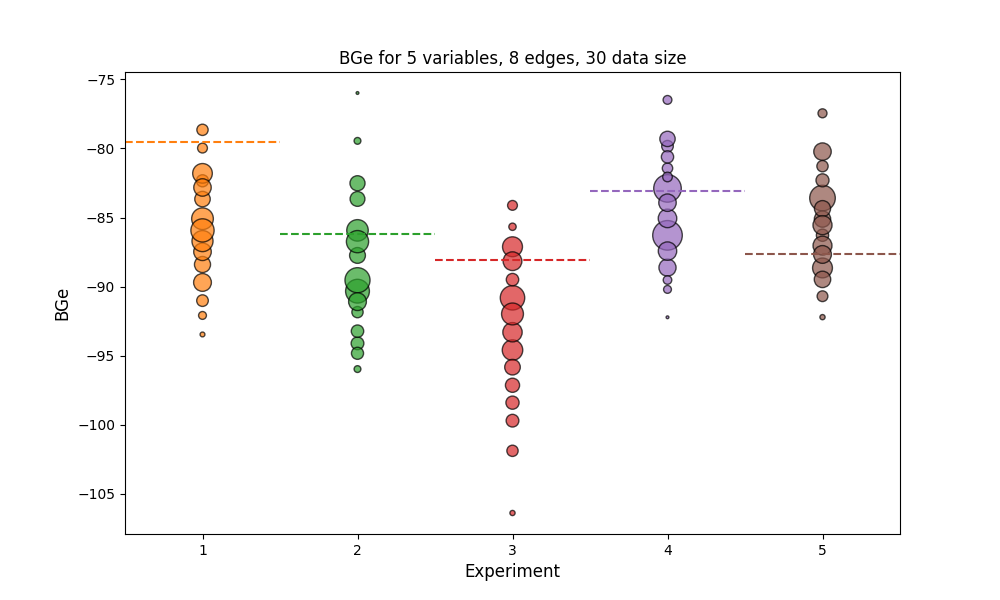
\includegraphics[width=\textwidth]{figures/BGe_5_8_30}
            \caption{BGe score distribution for Dataset 1.1.}
            \label{subfig:bge_score_5_8_30}
        \end{subfigure}
        \begin{subfigure}{0.48\textwidth}
            \centering
            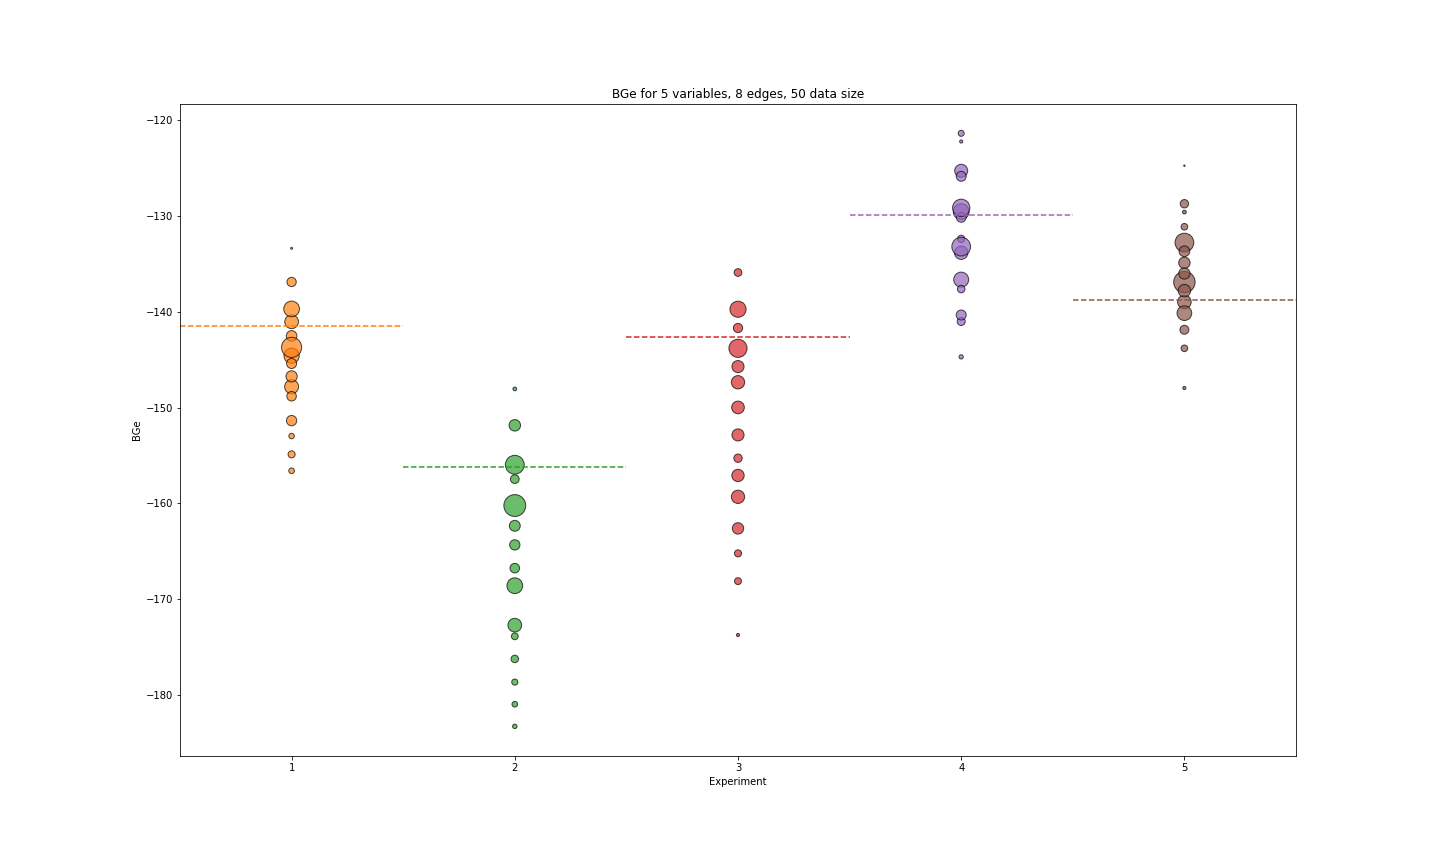
\includegraphics[width=\textwidth]{figures/BGe_5_8_50}
            \caption{BGe score distribution for Dataset 1.2.}
            \label{subfig:bge_score_5_8_50}
        \end{subfigure}
        \hfill
        \begin{subfigure}{0.48\textwidth}
            \centering
            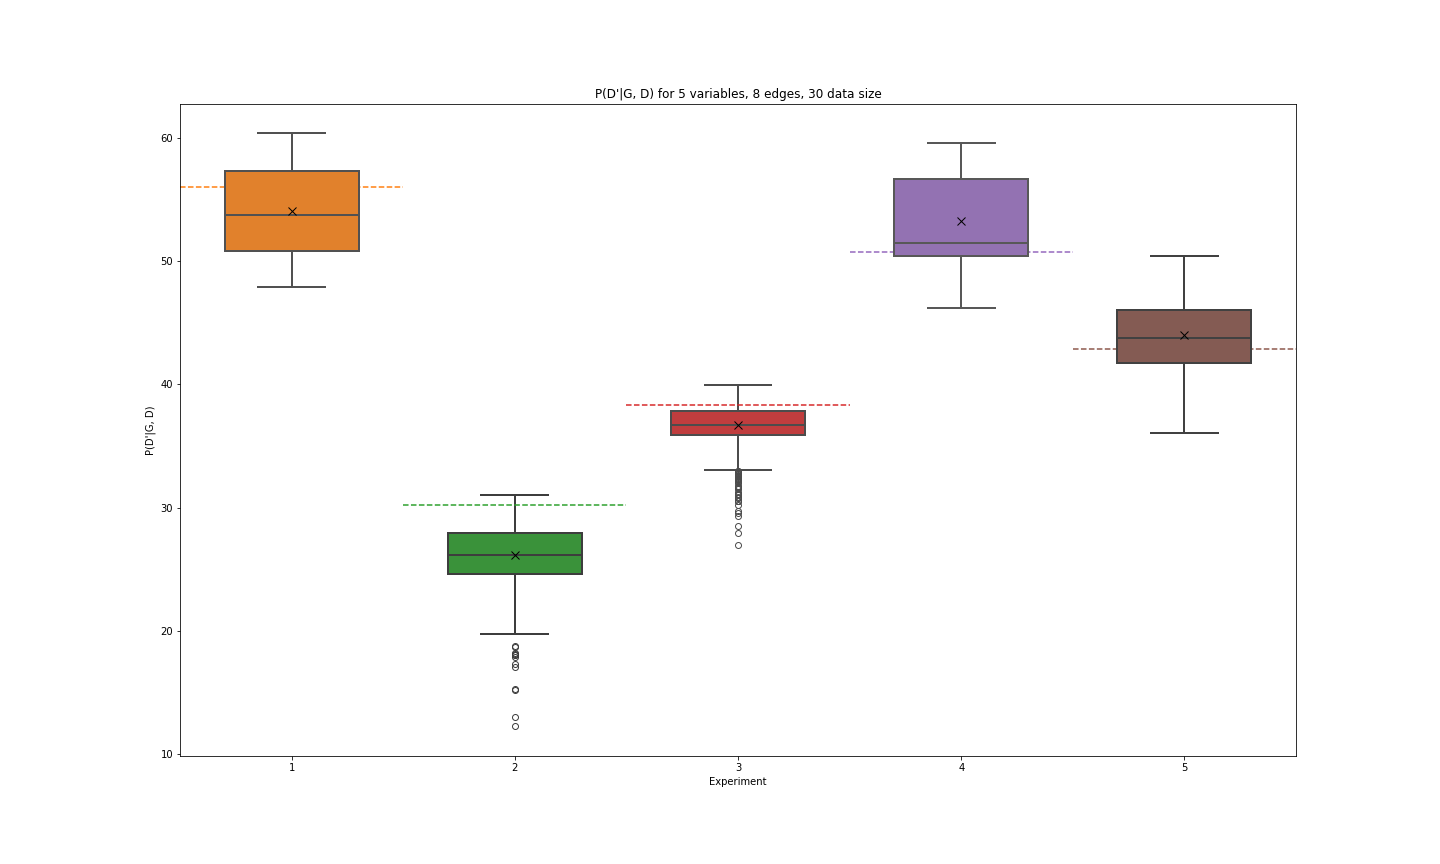
\includegraphics[width=\textwidth]{figures/P_d_prime_5_8_30}
            \caption{Held-out likelihood for Dataset 1.1.}
            \label{subfig:p_d_5_8_30}
        \end{subfigure}
        \begin{subfigure}{0.48\textwidth}
            \centering
            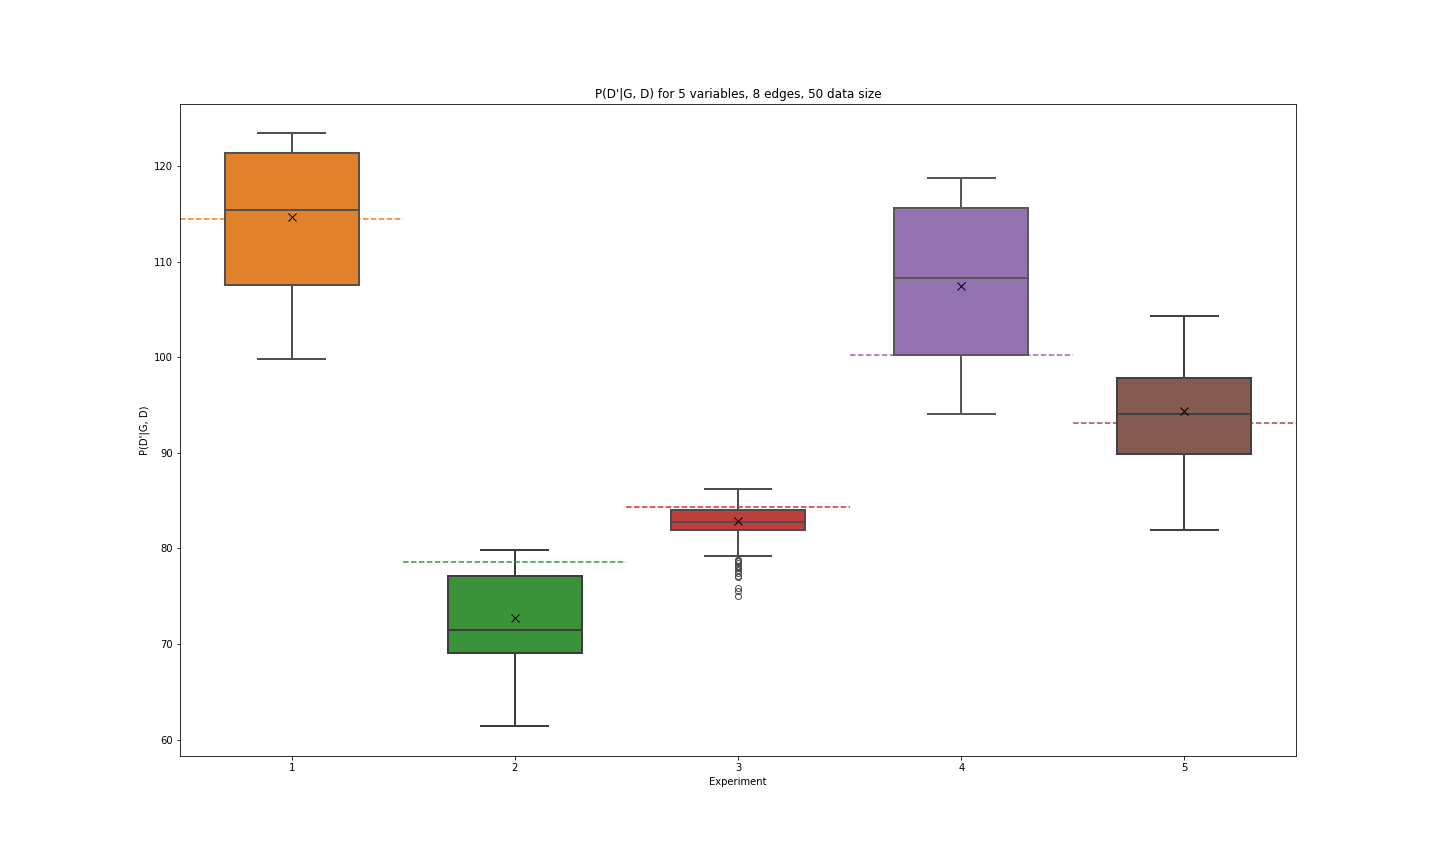
\includegraphics[width=\textwidth]{figures/P_d_prime_5_8_50}
            \caption{Held-out likelihood for Dataset 1.2.}
            \label{subfig:p_d_5_8_50}
        \end{subfigure}
        \caption{BGe score distribution and held-out likelihood results for Dataset 1.1 and Dataset 1.2. For Fig.~\ref{subfig:bge_score_5_8_30} and~\ref{subfig:bge_score_5_8_50}, the x-axis represents the experiment and the y-axis
        represents the BGe score distribution. For Fig.~\ref{subfig:p_d_5_8_30} and~\ref{subfig:p_d_5_8_50}, the x-axis
        represents the experiment and the y-axis represents the held-out likelihood.}
        \label{fig:illustration_5_8}
    \end{figure*}

    \begin{figure*}[h]
        \centering
        \begin{subfigure}{0.32\textwidth}
            \centering
            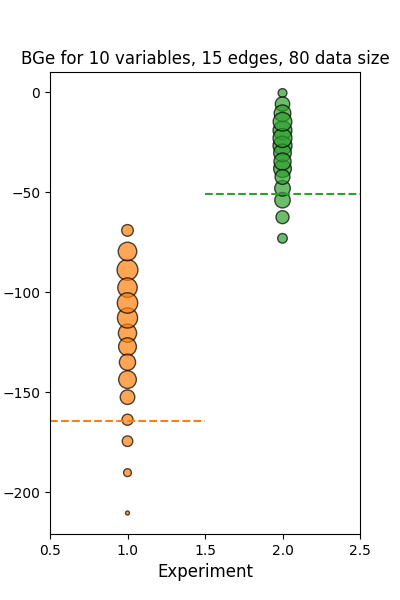
\includegraphics[width=\textwidth]{figures/BGe_10_15_80}
            \caption{BGe score distribution for Dataset 2.1.1.}
            \label{fig:bge_score_10_15_80}
        \end{subfigure}
        \begin{subfigure}{0.32\textwidth}
            \centering
            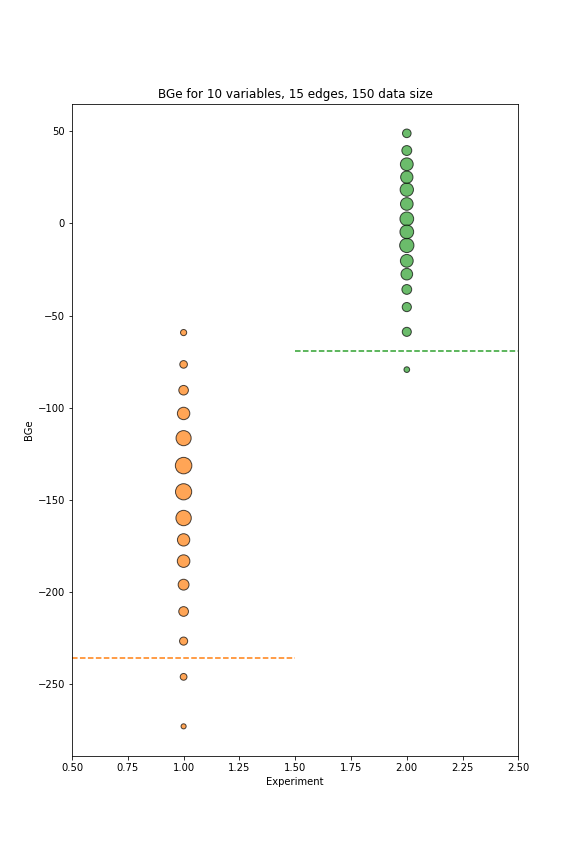
\includegraphics[width=\textwidth]{figures/BGe_10_15_150}
            \caption{BGe score distribution for Dataset 2.1.2.}
            \label{fig:bge_score_10_15_150}
        \end{subfigure}
        \begin{subfigure}{0.32\textwidth}
            \centering
            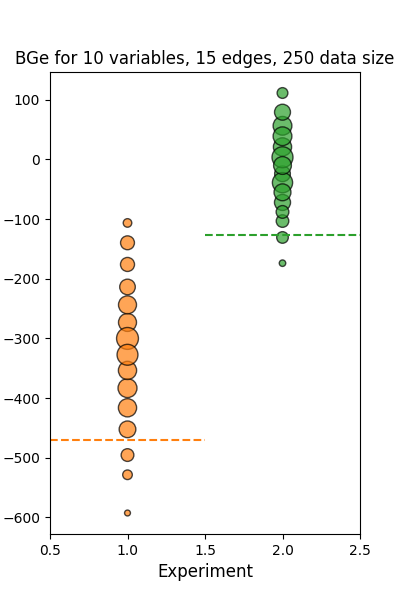
\includegraphics[width=\textwidth]{figures/BGe_10_15_250}
            \caption{BGe score distribution for Dataset 2.1.3.}
            \label{fig:bge_score_10_15_250}
        \end{subfigure}
        \hfill
        \begin{subfigure}{0.32\textwidth}
            \centering
            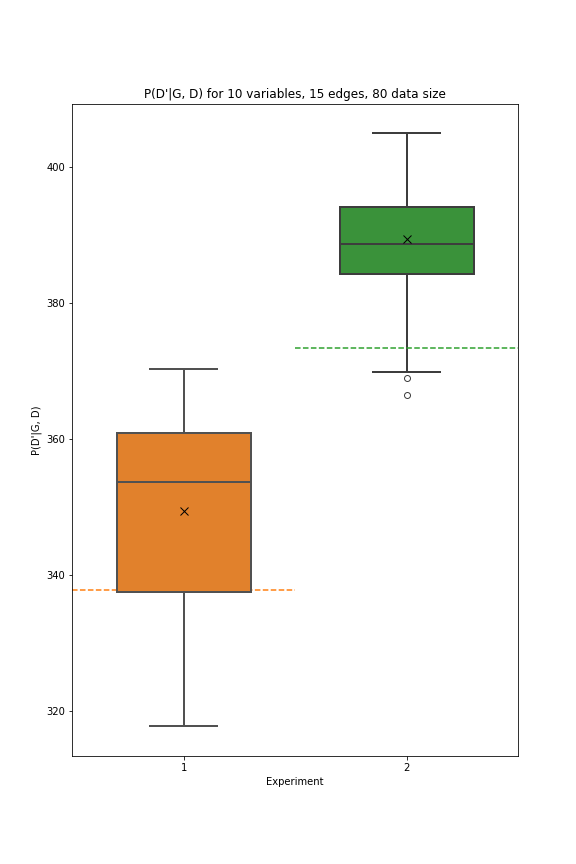
\includegraphics[width=\textwidth]{figures/P_d_prime_10_15_80}
            \caption{Held-out likelihood for Dataset 2.1.1.}
            \label{fig:p_d_10_15_80}
        \end{subfigure}
        \begin{subfigure}{0.32\textwidth}
            \centering
            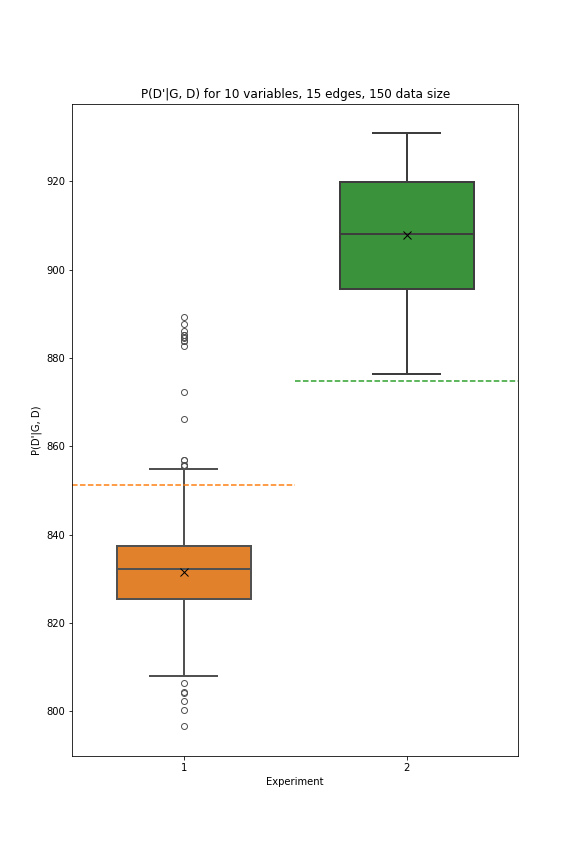
\includegraphics[width=\textwidth]{figures/P_d_prime_10_15_150}
            \caption{Held-out likelihood for Dataset 2.1.2.}
            \label{fig:p_d_10_15_150}
        \end{subfigure}
        \begin{subfigure}{0.32\textwidth}
            \centering
            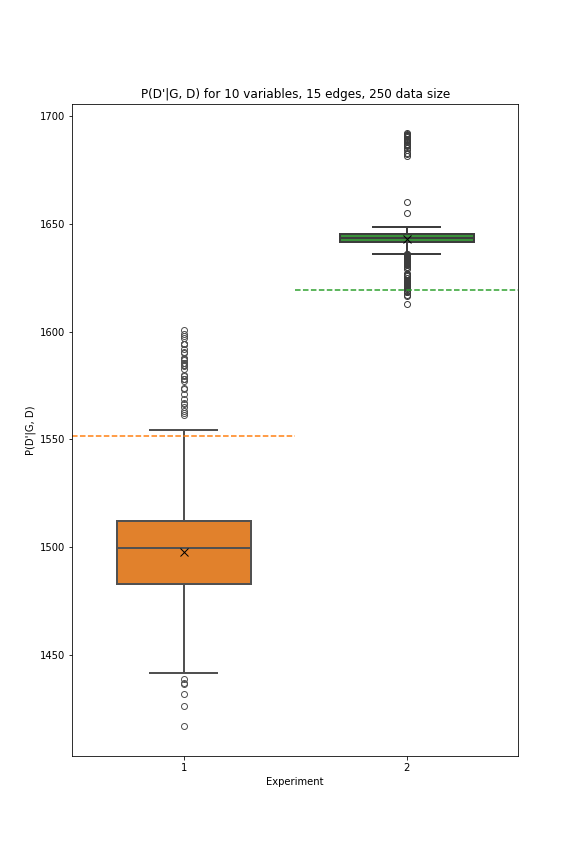
\includegraphics[width=\textwidth]{figures/P_d_prime_10_15_250}
            \caption{Held-out likelihood for Dataset 2.1.3.}
            \label{fig:p_d_10_15_250}
        \end{subfigure}
        \caption{BGe score distribution and held-out likelihood for Dataset 2.1.1: Fig.~\ref{fig:bge_score_10_15_80} and~\ref{fig:p_d_10_15_80}, Dataset 2.1.2: Fig.~\ref{fig:bge_score_10_15_150} and~\ref{fig:p_d_10_15_150}, and Dataset
        2.1.3: Fig.~\ref{fig:bge_score_10_15_250} and~\ref{fig:p_d_10_15_250}. X-axis represents the experiment and
        the y-axis represents the BGe score distribution and held-out likelihood.}
        \label{fig:illustration_10_15}
    \end{figure*}

    \subsubsection{E-SHD and AUROC and AUPRC}

    Since the number of experiments for Dataset 2 is small we will include the results for these metrics in a
    table instead of plots. However, for Dataset 1, Fig.~\ref{fig:metrics_dataset_1} shows the results for E-SHD, AUROC,
    and AUPRC metrics. The x-axis represents the dataset size and the y-axis represents the metric under discussion.

    \begin{figure*}[h]
        \centering
        \begin{subfigure}{0.98\textwidth}
            \centering
            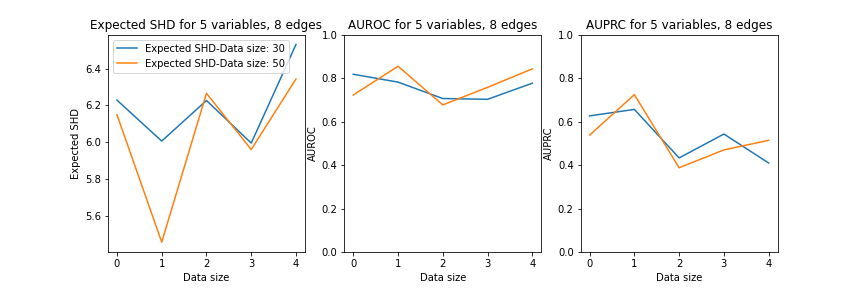
\includegraphics[width=\textwidth]{figures/expected_0_5_8}
            \caption{E-SHD, AUROC, AUPRC results for Dataset 1.1 and Dataset 1.2.}
            \label{fig:eshd_5_8}
        \end{subfigure}
        \caption{E-SHD, AUROC, and AUPRC results for Dataset 1.1 and Dataset 1.2. Note that in each figure, different colors show results for different data
        sizes.}
        \label{fig:metrics_dataset_1}
    \end{figure*}

    Table~\ref{tab:metrics_dataset_2} shows the results for E-SHD, AUROC, and AUPRC metrics for Dataset 2.1 and Dataset 2.2.

    \begin{table}[h]
        \centering
        \begin{tabular}{|l|c|c|c|}
            \hline
            \textbf{Dataset} & \textbf{E-SHD} & \textbf{AUROC} & \textbf{AUPRC} \\
            \hline
            Dataset 2.1.1    & 29.316, 28.067 & 0.564, 0.753   & 0.223, 0.299   \\
            Dataset 2.1.2    & 26.721, 28.209 & 0.737, 0.629   & 0.415, 0.494   \\
            Dataset 2.1.3    & 29.772, 25.321 & 0.563, 0.659   & 0.230, 0.309   \\
            Dataset 2.2.1    & 28.468, 25.75  & 0.580, 0.700   & 0.312, 0.467   \\
            Dataset 2.2.2    & 30.67, 29.997  & 0.520, 0.513   & 0.358, 0.363   \\
            \hline
        \end{tabular}
        \caption{E-SHD, AUROC, and AUPRC results for Dataset 2.1 and Dataset 2.2.}
        \label{tab:metrics_dataset_2}
    \end{table}


    \section{Conclusion}\label{sec:conclusion}
    \vspace*{-3mm}

    To start with the conclusion, we should firstly start with the comparisons of the BGe scores, and held-out
    likelihoods. Let's firstly start with Fig.~\ref{fig:illustration_5_8}, from the distribution of the BGe scores and
    the ground truth BGe score, we can see that the samples graphs are closely aligned with the ground truth graph
    in terms of BGe score. This is a good indication that the proposed approach is able to learn the structure of the
    graph well.

    Furthermore, the held-out likelihood results show that the learned distribution is able to generalize well for the
    held-out dataset. Although the alignment is not perfect, but considering the fact that the size of data $\mathcal{D}$
    is small, the results are promising.

    In comparison between results for different data sizes, we can see that in Fig.~\ref{subfig:bge_score_5_8_50}
    has a better alignment with the ground truth BGe score compared to Fig.~\ref{subfig:bge_score_5_8_30}. This
    clearly shows that this model is dependent on the size of the input data.

    Moving forward to Fig.~\ref{fig:p_d_10_15_80} to Fig.~\ref{fig:p_d_10_15_250}, we can see that the held-out
    likelihood results are not as consistent as for Dataset 1. This can show that although increasing the size of
    the data results in more concentrated posterior distribution, the distribution is not close enough to the ground
    truth. This could be due to the complexity of the graph structure and the size of the data.

    Mooving to E-SHD, AUROC, and AUPRC results, we can see that although the results for E-SHD is not promising,
    evaluated AUROC and AUPRC results show that for a less complex graph, AUROC is higher compared to AUPRC which shows
    consistency with theoretical analysis. However, for a more complex graph, the results are not as promising. This
    reasoning is consistent for Dataset 2 as well.


    While the proposed approach showed promising results compared to traditional methods, there remains room for
    improvement. Addressing computational limitations and exploring better mechanisms for handling complex graph
    structures could enhance scalability and robustness. These findings lay a solid foundation for further
    advancements in Bayesian structure learning using GFlowNets.


    \section{Future Work}\label{sec:future_work}
    \vspace*{-3mm}

    This project was a great opportunity to understand the recent advancements in the field of Bayesian Structure
    Learning. We have implemented the proposed approach in~\cite{deleu2022daggflownet} and conducted experiments to
    evaluate the performance of the proposed approach. We have used synthetic datasets to evaluate the performance of
    the proposed approach on graphs with different complexities and sizes. Numerous evaluation metrics were used to
    evaluate the performance of this approach. However, due to the scale of this project, we could not further
    explore the following directions and these could be suggestions for future work:

    \begin{itemize}
        \item \textbf{Real-world Datasets:} In this project, we used synthetic datasets to evaluate the performance of
        the proposed approach. However, it would be interesting to evaluate the performance of the proposed approach
        on real-world datasets. This could give us a better understanding of the robustness of the proposed approach
        in real-world scenarios.
        \item \textbf{Comparison with other Approaches:} In this project, we have implemented the proposed approach
        in~\cite{deleu2022daggflownet} and conducted experiments to evaluate the performance of the proposed approach.
        However, it would be interesting to compare the performance of the proposed approach with other approaches in
        the field of Bayesian Structure Learning.
        \item \textbf{Hyperparameter Tuning:} In this project, we have used a set of hyperparameters for the
        experiments. However, it would be interesting to conduct experiments with different hyperparameters to
        evaluate the performance of the proposed approach with different hyperparameters.
        \item And lastly, to our regret, we planned performing experiments on larger graphs included in
        Table~\ref{tab:future_dataset}, however because of the limited time and resources we had in hand,
        further exploration of these datasets was not possible.
    \end{itemize}

    \begin{table}[h]
        \centering
        \begin{tabular}{|l|c|c|c|}
            \hline
            \textbf{Dataset} & \textbf{Nodes} & \textbf{Average \# Edges} & \textbf{Data Size} \\
            \hline
            Dataset 3.1      & 15             & 45                        & 150                \\
            Dataset 3.2      & ---            & ---                       & 250                \\
            Dataset 3.3      & ---            & ---                       & 500                \\
            \hline
        \end{tabular}
        \caption{Datasets that could be used for future work.}
        \label{tab:future_dataset}
    \end{table}


    \pagebreak
    \newpage
    \clearpage
    \bibliographystyle{ieee_fullname}
    \bibliography{references}

    \makeappendix

    \appendix

    \counterwithin*{equation}{section}
    \renewcommand\theequation{\thesection\arabic{equation}}


    \section{Detailed Balance Condition}\label{app:detailed_balance}
    \vspace*{-3mm}

    In this section, as with the original paper (equations were taken from the original paper), we will prove the detailed balance condition
    for the proposed approach.

    Suppose all states are complete states excpet the terminal state $s_f$. Denote $P_F$ and $P_B$ as the forward
    and backward transition probabilities, respectively --- this is for simplifying the notation. The detailed balance
    condition according to~\cite{bengio2023gflownetfoundations} (Def. 17) is given by:
    \begin{equation}
        F(s_t)P_F(s_{t+1} \mid s_t) = F(s_{t+1})P_B(s_t \mid s_{t+1})
        \label{eq:detailed_balance_app}
    \end{equation}
    In the case where all the states are complete, we also know that (\cite{bengio2023gflownetfoundations} Def. 16):
    \[
        P_F(s_f \mid s_t) \coloneq \frac{F(s_t \to s_f)}{\sum_{s \in \text{Ch}(s_t)} F(s_t \to s)} = \frac{R(s_t)}{F(s_t)}
        \LeftRightArrow F(s_t) = \frac{R(s_t)}{P_F(s_f \mid s_t)},
    \]
    where $F(s \to s')$ represents the flow from state $s$ to  $s'$. Replacing $F(.)$ in Eq.~\eqref{eq:detailed_balance_app}
    yields:
    \begin{equation}
        R(s_t)P_F(s_{t+1} \mid s_t)P_F(s_f \mid s_{t+1}) = R(s_{t+1})P_B(s_t \mid s_{t+1})P_F(s_f \mid s_t).
        \label{eq:detailed_balance_app2}
    \end{equation}
    This concludes the proof of the detailed balance condition.


    \section{Masking Operation}\label{app:masking}
    \vspace*{-3mm}

    In this section we will explain the masking operation used in~\cite{deleu2022daggflownet} to enforce the acyclicity
    constraint. Authors suggested an online update of the mask matrix to avoid unnecessary computation of this mask
    from scratch for each graph.

    Firstly, we should introduce \textit{Transitive Closure} and $G^T$ which is the transpose of the graph $G$.
    Transpose of a directed graph $G$ is another directed graph on the same set of vertices with all of the edges
    reversed. Denote this graph as $G^T$. Furthermore, the transitive closure of a directed graph $G$ is a graph
    such that there is an edge from $i$ to $j$ in $T$ if and only if there is a directed path from $i$ to $j$ in
    $G$. If we denote the adjacency matrix of $G$ as $A$, and Adjacency matrix of Transitive closure of $G^T$ as $T$,
    then the mask matrix $m$ is defined as:
    \[
        m = A + T,
    \]
    where $+$ is the element-wise addition.
    Each element of this matrix, if 0, indicates that an edge between the corresponding nodes is allowed, and if 1,
    indicates that an edge between the corresponding nodes is not allowed. The intuition behind this operation is
    that if an edge is in the original matrix, it cannot be added again (adjacency matrix part) and if there is a
    directed path in the original matrix from $i$ to $j$ --- implying that there is an edge from $j$ to $i$ in the
    transitive closure of the transposed graph --- we cannot add an edge from $j$ to $i$ (transitive closure part).
    Note that the diagonal elements of the adjacency matrix which are corresponding to self-loops are set to 1 in $T$
    by convention.

    Suppose we have a graph $G_t$ and its respective mask $m_t$. This mask is made of two parts, Adjacency matrix of
    the graph $A_t$ and transitive closure of $G_t^T$ denoted as $T_{t}$. For adding an edge $i$ to $j$ to the
    graph (supposed this edge is allowed), the new adjacency matrix could be calculated easily. Now for $T_{t+1}$:
    Take the column corresponding to index of $j$ in $T_t$ and the row corresponding to index of $i$ in $T_t$ and
    perform outer product operation on $C_j$ and $R_i$ to get a new matrix $\hat{T}_{t+1}$. $T_{t+1}$ is then
    calculated as $T_t + \hat{T}_{t+1}$.

    The intuition behind this is: $C_j$ is the nodes that have a directed path to $j$ and $R_i$ is the nodes that
    $i$ have a directed path to. The outer product operation will result in a matrix where the element $[a, b]$ is
    non-zero if there is a directed path from $b$ to $a$ in the original matrix and thus, we cannot add an edge from
    $a$ to $b$. Fig.~\ref{fig:masking} shows the masking operation for a simple graph, and you can follow these
    explanations on this figure to better understand the operation.

    \begin{figure}[h]
        \centering
        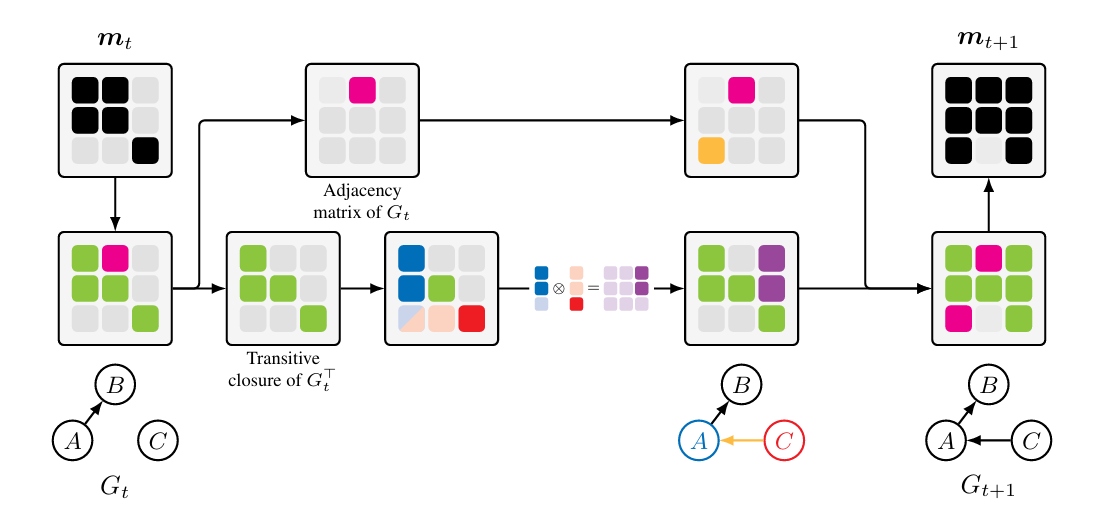
\includegraphics[width=0.92\textwidth]{figures/masking}
        \caption{Masking operation for a simple graph. Figure is taken from the original paper~\cite{deleu2022daggflownet}.}
        \label{fig:masking}
    \end{figure}


    \section{Linear Attention Mechanism}\label{app:linear_attention}
    \vspace*{-3mm}

    In this section, we will explain the linear attention mechanism used in the proposed approach. The linear attention
    mechanism is a variant of the self-attention mechanism used in transformers. The self-attention mechanism is
    computationally expensive as it scales quadratically with the input size. The linear attention mechanism on the
    other hand, relies on the following equations:
    \begin{equation}
        Q = XW_Q, \quad K = XW_K, \quad V = XW_V, LinAttn_k(X) = \frac{\sum_{j=1}^{d^2}
            \left(\phi(Q_k)^T\phi(K_j)\right)V_j}{\sum_{j=1}^{d^2} \phi(Q_k)^T\phi(K_j)},
        \label{eq:linear_attention}
    \end{equation}

    where $Q$, $K$, and $V$ are the query, key, and value matrices, respectively. $W_Q$, $W_K$, and $W_V$ are the
    weight matrices for the query, key, and value, respectively. $\phi$ is a non-linear feature map, and $d$ is the
    number of nodes in the graph.

    To better understand the linear characteristic of time complexity, suppose for on edge addition, we want to
    perform the calculation. The time complexity is constant with respect to the size of the embedding space. Thus,
    for $d^2$ edges, the time complexity is $O(d^2)$.


    \section{Data Generation Process}\label{app:data_generation}
    \vspace*{-3mm}

    The data Generation Process is mostly based on the original paper which itself is based on the work of~\cite{erdos1960evolutionrandomgraphs}.
    The process is as follows:

    \begin{enumerate}
        \item Sample a DAG based on prior probability $P(G)$ that is based on the model present by~\cite{erdos1960evolutionrandomgraphs}.
        This model is a modular prior function that considers the probability of existence of an edge between two
        nodes independently. Generation of such graph is based on a bionomial distribution with expected value of $2e$
        where $e$ is the number of edges. In the data generation process, we make sure that the graph is acyclic and
        the expected number of edges in the final graph is $e$.

        Firstly, we sample a $d \times d$ matrix $A$ where each element $A_{ij}$ is sampled from a Binomial
        distribution with
        \begin{equation}
            p = \frac{2e}{d(d-1)}.
            \label{eq:binomial}
        \end{equation}
        Then, elements on and above diagonal are thrown away to make sure the adjacency matrix is lower-triangular.
        This lower-triangular matrix is acyclic. Then, for relabeling purposes, rows and columns are permuted with
        the same random permutation --- this is a common convention for relabeling a graph and does not change the
        structure of the graph.
        The expected number of edges in the final graph is $e$ because the expected number of edges in the sampled
        matrix $A$ is $2e$ and we throw away half of the elements.

        \item After acquireing a dag, we sample its parameters
        based on a normal distribution with mean 0 and standard deviation 1. We also account for a noise term that
        is considered to be zero in the experiments, thus, the equation of the graph would be:
        \begin{equation}
            X_j = \sum_{i \in \text{Pa}_G(X_j)} \theta_{ij}X_i + \epsilon_j,
            \label{eq:graph}
        \end{equation}
        where $\theta_{ij} \sim \mathcal{N}(0, 1)$ and $\epsilon_j \sim \mathcal{N}(0, 0.01)$. Note that $X_j$ is the
        mean of the normal distribution that the data for node $j$ is sampled from. The variance of this normal
        distribution is considered to be 0.1 for all nodes.

        \item Now that we have the graph and its parameters, we sample $\mathcal{D}$ using ancestral sampling.
    \end{enumerate}


    \section{Training Loop}\label{app:training_loop}
    \vspace*{-3mm}

    In this section, we will explain the training loop used in the experiments. The training loop is based on the
    training loop in the original paper. The training loop is depicted in Alg.~\ref{alg:training_loop}.
    We start by initializing the environment, replay buffer, and model parameters.
    During each iteration, actions are sampled based on the current policy and an exploration parameter ($\epsilon$
    ), these actions are then executed in the environment, and the resulting transitions are stored in the replay
    buffer. After a prefill
    phase, batches of transitions are sampled from the buffer to update the model's parameters. The exploration
    parameter is adjusted dynamically. Once training is complete, the posterior distribution of graphs is estimated,
    this estimation is done using sampling from the learned distribution. Finally, evaluation results, and
    vbvariables are saved to disk.


    \begin{algorithm}[H]
        \caption{Training Loop for DAG-GFlowNet}
        \begin{algorithmic}[1]
            \Require Environment and GFlowNet initialized with parameters
            \Require Replay buffer initialized with capacity
            \Require Exploration schedule $\epsilon$ defined
            \State Initialize random seed and keys
            \State Reset environment to obtain initial observations

            \For{iteration $= 1$ to \texttt{prefill} + \texttt{num\_iterations}}
                \State \textbf{Sample actions:} Compute actions using policy with exploration parameter $\epsilon$
                \State \textbf{Execute actions:} Perform actions in the environment to obtain:
                \begin{itemize}
                    \item Next observations
                    \item Delta scores
                    \item Termination flags (\texttt{dones})
                \end{itemize}
                \State \textbf{Update Replay Buffer:} Store transitions (observations, actions, next observations, rewards, and dones) in the buffer
                \State Update observations with next observations

                \If{iteration $\geq$ \texttt{prefill}}
                    \State \textbf{Sample Batch:} Randomly sample a batch from the replay buffer
                    \State \textbf{Update Parameters:} Perform one optimization step using sampled batch
                \EndIf

                \State Update $\epsilon$ using exploration schedule
                \State Log progress (loss, exploration rate, etc.)
            \EndFor

            \State \textbf{Posterior Estimate:} Compute posterior distribution of graphs using the trained GFlowNet
            \State \textbf{Compute Metrics:} Evaluate the expected SHD, expected edges, and other threshold-based metrics
            \State \textbf{Save Results:} Store the model, replay buffer, posterior samples, and evaluation metrics to disk
        \end{algorithmic}\label{alg:training_loop}
    \end{algorithm}

    \subsection{Reinforcement Learning Concepts}\label{app:rl_concepts}
    \vspace*{-3mm}


    In reinforcement learning (RL), the \textbf{environment} represents the external system or task that the agent
    interacts with to learn a policy. The environment provides the agent with:
    \begin{itemize}
        \item \textbf{State:} A representation of the current status or configuration of the system.
        \item \textbf{Action space:} The set of possible actions the agent can take to influence the environment.
        \item \textbf{Transition dynamics:} Rules governing how the environment evolves in response to the agent's actions.
        \item \textbf{Reward signal:} Feedback used by the agent to evaluate the effectiveness of its actions and guide future decisions.
    \end{itemize}


    In this work, the environment is designed to model the structure learning problem as a graph generation task. It
    provides observations representing partial or complete graph structures, accepts actions that modify the graph (
    e.g., adding or removing edges), and computes rewards based on changes in the graph's score. This setup enables the
    GFlowNet agent to explore and learn graph structures that maximize the overall objective, aligning RL principles
    with the requirements of structure learning.


%\begin{thebibliography}{99}
%\end{thebibliography}

\end{document}
